\documentclass[11pt, a4paper]{article}

\usepackage{amssymb}
\usepackage{listings}
\usepackage[nodayofweek]{datetime}
\usepackage{graphicx}
\usepackage[breaklinks]{hyperref}
\usepackage[all]{hypcap}

\setlength{\parindent}{0cm}
\setlength{\parskip}{0.4cm}

\begin{document}

\begin{titlepage}
\begin{center}
	\textsc{\huge MQP Title }\\[1cm]
	A Major Qualifying Project Report\\
	submitted to the Faculty of\\[0.7cm]
	\textsc{ \large Worcester Polytechnic Institute }\\[0.7cm]
	in partial fulfillment of\\
	the requirements for the degree of\\
	Bachelor of Science\\[1cm]
	by\\[1cm]
	~\hspace{2cm}\dotfill\hspace{2cm}~\\
	\textsc{\Large Michael Ficarra}\\[1cm]
	on\\[1cm]
	{\Large \today}\\
	\vfill
	\begin{flushright}
		\hspace{8cm}\dotfill \\
		\textsc{Daniel Dougherty}\\
		professor, project advisor\\
	\end{flushright}
\end{center}
\end{titlepage}

\pagenumbering{roman}

~\\
\vfill
\begin{abstract}
This paper describes a method, referred to as the chase, for generating minimal
models for a geometric theory. A minimal model for a theory is a model for
which there exists a homomorphism to any other model that can satisfy the
theory. These models are useful in solutions to problems in many practical
applications, including firewall configuration examination and access control
evaluation. Also described is a Haskell implementation of the chase and its
development process and design decisions.
\end{abstract}
\vfill
~\\
\newpage

\renewcommand{\contentsname}{Table of Contents}
\tableofcontents \newpage
\listoffigures \newpage
\listoftables \newpage

\pagenumbering{arabic}


% main paper sections
\section{Introduction}

	\textbf{ remove this? }

	This document details work done for a Major Qualifying Project at Worcester
	Polytechnic Institute by Michael Ficarra in partial fulfillment of the
	requirements for a Bachelor of Science degree in Computer Science.

	Section \ref{sec:technical_background} can be used as a reference for terms
	discussed in later sections. Appendices \ref{sec:appendix_glossary} and
	\ref{appendix_syntax_table} contain a glossary and syntax reference,
	respectively.

	\subsection{Goals}

		The two main goals of this Major Qualifying Project are:

		\begin{enumerate}
		\item to implement an algorithm known as ``the chase" accurately
		and with a well-defined, usable interface, and
		\item to use the chase implementation for a real-world
		application: generating models used in analysis of a specific protocol
		\end{enumerate}

		Secondary goals include implementing various optimizations and
		integrating the chase implementation into a program that can take
		advantage of the functionality it provides.

	\subsection{The Chase}

		\textbf{ this whole section needs some expanding still }

		\emph{The chase} is an algorithm used to find jointly minimal models
		(see \ref{sec:technical_background.minimal_models}) for a set of
		geometric logic formul{\ae}. Many common real-world problems can be
		expressed as a set of geometric logic formul{\ae} (see
		\ref{sec:technical_background.geometric_logic}). When these problems
		have an unbounded scope of possible solutions, the chase can be used to
		find the possible solutions that are interesting. This allows
		researchers to go through only models that represent a large set of
		models rather than testing each of the infinite number of models
		separately.

		To generate these jointly minimal models, the chase begins with a model
		$\mathbb{M}$ that has an empty domain and no facts. The chase goes
		through each formula $\sigma$ in the geometric theory $T$ such that
		$\mathbb{M} \not\models \sigma$ and alters $\mathbb{M}$ so that
		$\mathbb{M} \models \sigma$. Geometric formul{\ae} are implications of
		positive-existential formul{\ae} (see
		\ref{sec:technical_background.geometric_logic}). Positive-existential
		formul{\ae} have the useful property in that adding elements/facts to a
		model that satisfies one will never cause the model to no longer
		satisfy that formula. Because of this, the chase can keep adding to the
		model until all formul{\ae} are satisfied. The set of all models
		generated by this process is a jointly minimal set for the input theory
		$T$.

		The chase is nondeterministic over disjunctions. When a disjunction is
		encountered, a disjunct is chosen and the chase continues until it
		encounters another disjunct.

	\subsection{Chase Implementation}

		We will see in section \ref{sec:implementation} that, in a Haskell
		implementation of the chase, both disjuncts can be satisfied by forking
		the chase and returning a list containing the concatenation of the
		lists returned by the forks. In this way, we can deterministically
		calculate a set of jointly minimal models by using a naturally
		nondeterministic algorithm.

	\subsection{Application}

		Cryptographic protocol analysis is the particular application that is
		explored in section \ref{sec:application.strand_spaces}. In this
		application, protocols are modeled in the strand space formalism. Each
		role of every participant in a legal run of the protocol is modeled as
		a strand. The roles of a special participant that does not obey the
		rules of the protocol are called adversary strands (see
		\ref{sec:application.the_adversary}). These adversary strands consist
		of a series of nodes that send/receive messages to/from regular strands
		while manipulating those messages. Because the positions and actions of
		adversary strands are variable, there exists a large number of possible
		runs of a single protocol. It is prohibitive to test all of these to
		find if they break assumptions made about the properties of the
		protocol. The runs of this protocol can be represented as a geometric
		theory and passed to the chase to find minimal models. When minimal
		models are found, they can describe nearly all interesting ways that
		the adversaries can interact with regular strands. These models can
		then be analysed in a finite amount of time.

\section{Technical Background}
\label{sec:technical_background}

	\subsection{Vocabulary}

		A \emph{relation symbol}, often called a \emph{predicate}, can be any
		unique symbol. An \emph{arity} function takes a relation symbol as
		input and returns a non-negative integer. A \emph{vocabulary} is a
		construct containing a set of relation symbols and an arity function.

	\subsection{Models}

		A \emph{model} $\mathbb{M}$ for a vocabulary $\mathcal{V}$ is a
		construct that consists of:
		\begin{itemize}
		\item a set, denoted $|\mathbb{M}|$, called the \emph{universe} or \emph{domain} of $\mathbb{M}$
		\item for each pairing of a predicate $R$ of arity $k$ in $\mathcal{V}$, a relation $R^\mathbb{M}_k \subseteq |\mathbb{M}|$
		\end{itemize}
		The relation itself is a set of tuples of members from the universe.

		\begin{definition}
			Let $\mathbb{A}$ and $\mathbb{B}$ be models. $\mathbb{A}$ is a
			\emph{submodel} of $\mathbb{B}$ if
			\begin{itemize}
			\item $|\mathbb{A}| \subseteq |\mathbb{B}|$
			\item for each relation $R$, $R^\mathbb{A} \subseteq R^\mathbb{B}$

			That is, for each tuple $\vec a$ from $|\mathbb{A}|$, $\vec a \in
			R^\mathbb{A}$ implies  $\vec a \in R^\mathbb{B}$.
			\end{itemize}
		\end{definition}

	\subsection{First-order Logic}

		\emph{First-order logic}, also called \emph{predicate logic}, is a
		formal logic system. A first-order logic formula is defined inductively
		by the following:
		\begin{itemize}
		\item if $R$ is a relation symbol of arity $k$ and each of $x_0 \ldots x_{k-1} \in \vec{x}$ is a variable, then $R(\vec{x})$ is a formula, specifically an \emph{atomic formula}
		\item if $x$ and $y$ are variables, then $x = y$ is a formula
		\item $\top$ and $\bot$ are formul{\ae}
		\item if $\alpha$ is a formula, then $(\neg\alpha)$ is a formula
		\item if $\alpha$ and $\beta$ are formul{\ae}, then $(\alpha \wedge \beta)$ is a formula
		\item if $\alpha$ and $\beta$ are formul{\ae}, then $(\alpha \vee \beta)$ is a formula
		\item if $\alpha$ and $\beta$ are formul{\ae}, then $(\alpha \to \beta)$ is a formula
		\item if $\alpha$ is a formula and $x$ is a variable, then $(\forall\ x : \alpha)$ is a formula
		\item if $\alpha$ is a formula and $x$ is a variable, then $(\exists\ x : \alpha)$ is a formula
		\end{itemize}

		For our purposes, this logic system will not contain any constant
		symbols or function symbols which are commonly included in first-order
		logic. We will see in section
		\ref{sec:technical_background.geometric_logic} that these are
		unnecessary and can be replicated using other, allowed constructs.

		A shorthand notation may sometimes be used which omits either the left
		or right side of an implication and denotes ($\top \to \sigma$) and
		($\sigma \to \bot$) respectively. If $\alpha$ is a formula and
		$\vec{x}$ is a set of variables of size $k$, then $(\forall\ \vec{x} :
		\alpha)$ is $(\forall\ x_0 \ldots \forall\ x_{k-1} : \alpha)$. If
		$\alpha$ is a formula and $\vec{x}$ is a set of variables of size $k$,
		then $(\exists\ \vec{x} : \alpha)$ is $(\exists\ x_0 \ldots \exists\
		x_{k-1} : \alpha)$.

	\subsection{Variable Binding}

		The set of free variables in a formula $\sigma$, denoted $free(\sigma)$
		is defined inductively as follows:
		\begin{itemize}
		\item $free( R(x_0,\ldots,x_n) )$ = $\{x_0,\ldots,x_n\}$
		\item $free(\top)$ = $\emptyset$
		\item $free(\bot)$ = $\emptyset$
		\item $free(x = y)$ = $\{x,y\}$
		\item $free(\neg\alpha)$ = $free(\alpha)$
		\item $free(\alpha \wedge \beta)$ = $free(\alpha) \cup free(\beta)$
		\item $free(\alpha \vee   \beta)$ = $free(\alpha) \cup free(\beta)$
		\item $free(\alpha \to    \beta)$ = $free(\alpha) \cup free(\beta)$
		\item $free(\forall\ x : \alpha)$ = $free(\alpha)\ \backslash\ \{x\}$
		\item $free(\exists\ x : \alpha)$ = $free(\alpha)\ \backslash\ \{x\}$
		\end{itemize}
		A formula $\sigma$ is a \emph{sentence} if $free(\sigma) = \emptyset$.

	\subsection{Environment}

		An \emph{environment} $\lambda$ for a model $\mathbb{M}$ is a function
		from a set of variables $\vec v$ to $|\mathbb{M}|$. The syntax
		$\lambda_{[v \mapsto a]}$ denotes the environment $\lambda'(x)$ that
		returns $a$ when $x=v$ and returns $\lambda(x)$ otherwise.

	\subsection{Satisfiability}

		A model $\mathbb{M}$ is said to satisfy a formula $\sigma$ in an
		environment $\lambda$, denoted $\mathbb{M} \models_\lambda \sigma$ and
		read ``under $\lambda$, $\sigma$ is true in $\mathbb{M}$", when
		\begin{itemize}
		\item $\sigma$ is a relation symbol $R$ and $R(\lambda(a_0) , \ldots , \lambda(a_n)) \in \mathbb{M}$ where $a$ is a set of variables
		\item $\sigma$ is of the form $\neg\alpha$ and $\mathbb{M} \not\models_\lambda \alpha$
		\item $\sigma$ is of the form $\alpha\wedge\beta$ and both $\mathbb{M} \models_\lambda \alpha$ and $\mathbb{M} \models_\lambda \beta$
		\item $\sigma$ is of the form $\alpha\vee\beta$ and either $\mathbb{M} \models_\lambda \alpha$ or $\mathbb{M} \models_\lambda \beta$
		\item $\sigma$ is of the form $\alpha\to\beta$ and either $\mathbb{M} \not\models_\lambda \alpha$ or $\mathbb{M} \models_\lambda \beta$
		\item $\sigma$ is of the form $\forall\ x : \alpha$  and for every $x' \in |\mathbb{M}|$, $\mathbb{M} \models_{\lambda[x \mapsto x']} \alpha$
		\item $\sigma$ is of the form $\exists\ x : \alpha$  and for at least one $x' \in |\mathbb{M}|$, $\mathbb{M} \models_{\lambda[x \mapsto x']} \alpha$
		\end{itemize}
		The notation $\mathbb{M} \models \sigma$ (no environment specification)
		means that, under the empty environment $l$, $\mathbb{M} \models_l \sigma$.

		A model $\mathbb{M}$ satisfies a set of formul{\ae} $\Sigma$ under an
		environment $\lambda$ if for every $\sigma$ such that $\sigma \in
		\Sigma$, $\mathbb{M} \models_\lambda \sigma$. This is denoted as
		$\mathbb{M} \models_\lambda \Sigma$ and read ``$\mathbb{M}$ is a model
		of $\Sigma$".

	\subsection{Entailment}

		Given an environment $\lambda$, a set of formul{\ae} $\Sigma$ is said
		to \emph{entail} a formula $\sigma$ ($\Sigma \models_\lambda \sigma$)
		if the set of all models satisfied by $\Sigma$ under $\lambda$ is a
		subset of the set of all models satisfying $\sigma$ under $\lambda$.
		In other words, given a model $\mathbb{M}$, a set of formul{\ae}
		$\Sigma$, and a formula $\sigma$ such that $\Sigma \models \sigma$,
		whenever $\mathbb{M} \models \Sigma$, $\mathbb{M} \models \sigma$.

		The notation used for satisfiability and entailment is very similar, in
		that the operator used ($\models$) is the same, but they can be
		distinguished by the type of left operand.

	\subsection{Homomorphisms}

		A \emph{homomorphism from $\mathbb{A}$ to $\mathbb{B}$} is a function
		$h: |\mathbb{A}|\to|\mathbb{B}|$ such that, for each relation symbol
		$R$ and tuple $\langle a_0 , \ldots , a_n \rangle$, $\langle a_0 ,
		\ldots , a_n  \rangle \in R^\mathbb{A}$ implies $\langle h(a_0) ,
		\ldots , h(a_n) \rangle \in R^\mathbb{B}$. The identity function is a
		homomorphism from any model $\mathbb{M}$ to itself.

		%\begin{theorem}
		%	A homorphism $h: |\mathbb{M}| \to |\mathbb{N}|$
		%	is a composition of zero or more of the following functions:
		%	\begin{itemize}
		%	\item $addDomain(\omega):
		%		|\mathbb{M}| \to |\mathbb{M}| \cup \vec\omega$ where
		%		$\vec\omega$ is non-empty and each $\omega \in \vec\omega$ is a
		%		domain member not in $|\mathbb{M}|$
		%	\item $addFact:
		%		\mathbb{M} \to \mathbb{N}$ where $|\mathbb{M}| = |\mathbb{N}|$,
		%		for each fact $R^\mathbb{M}(\alpha_0,\ldots,\alpha_n)$, there
		%		exists an $R^\mathbb{N}(\alpha_0,\ldots,\alpha_n)$, and for
		%		each predicate $P \in \mathbb{N}$ there exists one or more
		%		facts $P^\mathbb{N}(\gamma_0,\ldots,\gamma_k)$
		%	\item $rename:
		%		\mathbb{M} \to \mathbb{N}$ where, for every
		%		$R^\mathbb{M}(\alpha_0,\ldots,\alpha_n)$ where $\alpha \in
		%		|\mathbb{M}|$, there exists an
		%		$R^\mathbb{N}(\eta(\alpha_0),\ldots,\eta(\alpha_n))$ where
		%		$\eta$ is a homomorphism
		%	\end{itemize}
		%\end{theorem}

		A homomorphism $h$ is also a \emph{strong homomorphism} if, for each
		relation symbol $R$ and tuple $\langle a_0 , \ldots , a_n \rangle$,
		$\langle a_0 , \ldots , a_n  \rangle \in R^\mathbb{A}$ if and only if
		$\langle h(a_0) , \ldots , h(a_n) \rangle \in R^\mathbb{B}$.

		The notation $\mathbb{M} \preceq \mathbb{N}$ means that there exists a
		homomorphism $h : \mathbb{M} \to \mathbb{N}$. $\preceq$ has the
		property that $\mathbb{A} \preceq \mathbb{B} \wedge \mathbb{B} \preceq
		\mathbb{C}$ implies $\mathbb{A} \preceq \mathbb{C}$. However,
		$\mathbb{M} \preceq \mathbb{N} \wedge \mathbb{N} \preceq \mathbb{M}$
		does not imply that $\mathbb{M} = \mathbb{N}$. For example, fix two
		models $\mathbb{M}$ and $\mathbb{N}$ that are equivalent except that
		$|\mathbb{N}| = |\mathbb{M}| \cup \omega$ where $\omega \not\in
		|\mathbb{M}|$. Both $\mathbb{M} \preceq \mathbb{N}$ and $\mathbb{N}
		\preceq \mathbb{M}$ are true, yet $\mathbb{M} \neq \mathbb{N}$.

		Given two models $\mathbb{M}$ and $\mathbb{N}$, when $\mathbb{M}
		\preceq \mathbb{N}$ and $\mathbb{N} \preceq \mathbb{M}$, $\mathbb{M}$
		and $\mathbb{N}$ are \emph{homomorphically equivalent}. Homomorphic
		equivalence between a model $\mathbb{M}$ and a model $\mathbb{N}$ is
		denoted $\mathbb{M} \simeq \mathbb{N}$.

		Given models $\mathbb{M}$ and $\mathbb{N}$ where $\mathbb{M} \preceq
		\mathbb{N}$ and a formula in positive-existential form $\sigma$, if
		$\mathbb{M} \models \sigma$ then $\mathbb{N} \models \sigma$.

		A homomorphism $h : \mathbb{A} \to \mathbb{B}$ is also an
		\emph{isomorphism} when $h$ is 1:1 and onto and the inverse function
		$h^{-1} : \mathbb{B} \to \mathbb{A}$ is a homomorphism.

	\subsection{Universal Models}
	\label{sec:technical_background.universal_models}

		\emph{Universal models}, also called \emph{universal} models, are models
		for a theory $\mathcal{T}$ with the special property that there exists a
		homomorphism from the universal model to any other model that satisfies
		$\mathcal{T}$. Intuitively, universal models have no unnecessary entities or
		relations and thus display the least amount of constraint necessary to
		satisfy the theory for which they are universal. Any model to which there
		exists a homomorphism from a universal model will have more constraints
		than the universal model.

		A set of models $\mathcal{M}$ is said to be \emph{jointly universal} for
		a set of formul{\ae} $\Sigma$ when, for every model $\mathbb{N}$ such
		that $\mathbb{N} \models \Sigma$, there exists a homomorphism from a
		model $\mathbb{M} \in \mathcal{M}$ to $\mathbb{N}$. It follows that any
		superset of a jointly universal set of models is also jointly universal.

		More than one universal model may exist for a given theory. Given a model
		$\mathbb{M}$ that is universal for a theory $\mathcal{T}$, any model $\mathbb{N}$
		such that $\mathbb{N} \simeq \mathbb{M}$ is also universal for $\mathcal{T}$.

		Not every theory must have a universal model. A simple example of this is
		the theory containing a single formula $\sigma$ where $\sigma$ contains
		a disjunction. There exists no single universal model for the formula $P
		\vee Q$ ($P$ and $Q$ are relations with arity $0$) because any model that
		satisfies both $P$ and $Q$ would not have a homomorphism to a model
		that satisfies the theory with only $P$ or $Q$ in its set of facts.
		However, the set containing a model $\mathbb{M}$ that contains $P$ in
		its set of facts and a model $\mathbb{N}$ that contains $Q$ in its
		set of fact would be \emph{jointly} universal.

	\subsection{Positive Existential Form}

		Formul{\ae} in \emph{positive existential form} are constructed using
		only conjunctions ($\wedge$), disjunctions ($\vee$), existential
		quantifications ($\exists$), tautologies ($\top$), contradictions
		($\bot$), equalities, and relations.

		\begin{theorem}
			\label{pef_theorem}
			The set of models of a sentence $\sigma$ is closed under homomorphisms
			if and only if $\sigma$ is logically equivalent to a positive
			existential formula $\varphi$.
		\end{theorem}

		\begin{proof}
			This is a well-known classical result in model theory. See
			\cite{ChangKeisler73}, section 5.2 for example.

			We will only use one direction of Theorem \ref{pef_theorem}: the
			fact that if a sentence is in positive-existential form then it is
			closed under homomorphisms. To keep this paper self-contained, we
			provide here a proof of this fact.

			It suffices to prove the following, more general, claim for
			positive-existential \emph{formul{\ae}}.

			\begin{quote}
				If $\sigma$ is a positive-existential formula, $\mathbb{M}$ is
				a model, $\lambda : [var] \to |\mathbb{M}|$ is an environment
				such that $\mathbb{M} \models_\lambda \sigma$, and $h$ is a
				homomorphism $h : |\mathbb{M}| \to |\mathbb{M}'|$, then
				$\mathbb{M}' \models_{h\circ\lambda} \sigma$.
			\end{quote}

			We prove this by induction over formul{\ae}.

			When $\sigma$ is an atomic formula $R(x_0,\ldots,x_n)$, we know
			that $R(\lambda(x_0),\ldots,\lambda(x_n)) \in \mathbb{M}$ and by
			the definition of a homomorphism
				\[
				R((h(\lambda(x_0)),\ldots,(h(\lambda(x_n))) \in \mathbb{M}'
				\]
			That is,
				\[
				R((h\circ\lambda)(x_0),\ldots,(h\circ\lambda)(x_n)) \in \mathbb{M'}
				\]
			as desired.

			When $\sigma$ is $x=y$, we know that $\lambda(x) = \lambda(y)$, so
			$h(\lambda(x))$ must be $h(\lambda(y))$.

			When $\sigma$ is $\bot$, there exists no $\lambda$ such that
			$\mathbb{M} \models_\lambda \bot$, so the hypothesis of our claim
			never holds, which causes our claim to always hold.

			When $\sigma$ is $\top$, we know that $\mathbb{M} \models_\lambda
			\top$ and by the induction hypothesis, $\mathbb{M}'
			\models_{h\circ\lambda} \top$.

			When $\sigma$ is $\alpha \wedge \beta$, we know that $\mathbb{M}
			\models_\lambda \alpha$ and by the induction hypothesis
			$\mathbb{M}' \models_{h\circ\lambda} \alpha$. We also know that
			$\mathbb{M} \models_\lambda \beta$ and by the induction hypothesis
			$\mathbb{M}' \models_{h\circ\lambda} \beta$. By the definition of
			conjunction, because $\mathbb{M}' \models_{h\circ\lambda} \alpha$
			and $\mathbb{M}' \models_{h\circ\lambda} \beta$, we know that
			$\mathbb{M}' \models_{h\circ\lambda} \alpha \wedge \beta$.

			When $\sigma$ is $\alpha \vee \beta$, we know that if $\mathbb{M}
			\models_\lambda \alpha$, by the induction hypothesis $\mathbb{M}'
			\models_{h\circ\lambda} \alpha$. We also know that if $\mathbb{M}
			\models_\lambda \beta$, by the induction hypothesis $\mathbb{M}'
			\models_{h\circ\lambda} \beta$. By the definition of disjunction,
			because $\mathbb{M}' \models_{h\circ\lambda} \alpha$ or
			$\mathbb{M}' \models_{h\circ\lambda} \beta$, we know that
			$\mathbb{M}' \models_{h\circ\lambda} \alpha \vee \beta$.

			When $\sigma$ is $\exists\ \vec x : \alpha$, we know that
			$\mathbb{M} \models_\lambda \exists\ x : \alpha$, and want to prove
			that $\mathbb{M}' \models_{h\circ\lambda} \exists\ x : \alpha$.
			There is a $d \in |\mathbb{M}|$ such that $\mathbb{M}
			\models_{\lambda[x\mapsto d]} \alpha$. By our induction
			hypothesis, $\mathbb{M}' \models_{h\circ(\lambda[x\mapsto d])}
			\alpha$. This is equivalent to $\mathbb{M}'
			\models_{(h\circ\lambda)[x\mapsto h(d)]} \alpha$.
		\end{proof}

		\begin{corollary}
			If $\mathbb{M}$ is a submodel of $\mathbb{N}$, $\sigma$ is a
			positive-existential formula, and $\mathbb{M} \models \sigma$, then
			$\mathbb{N} \models \sigma$.
		\end{corollary}

		\begin{proof}
			If $\mathbb{M}$ is a submodel of $\mathbb{N}$ the inclusion
			function from $\mathbb{M}$ to $\mathbb{N}$ is a homomorphism.
		\end{proof}

	\subsection{Geometric Logic}
	\label{sec:technical_background.geometric_logic}

		\emph{Geometric logic} formul{\ae} are implicitly universally
		quantified implications between positive existential formul{\ae}. More
		specifically, a geometric logic formula is of the form
			\[
			\forall\ \vec{x} : F_L \to F_R
			\]
		where $\vec{x} = free(F_L) \cup free(F_R)$, $free$ is the function that
		returns the set of all free variables for a given formula, and both
		$F_L$ and $F_R$ are first-order logic formul{\ae} in positive
		existential form.

		A set of geometric logic formul{\ae} is called a \emph{geometric
		theory}.

		It is convention to treat a positive existential formula $\sigma$ as
		$\top \to \sigma$ when expecting a geometric logic formula. It is also
		convention to treat a negated positive existential formula $\neg\sigma$
		as $\sigma \to \bot$.


		\subsubsection{Examples}
		\label{sec:technical_background.geometric_logic.examples}

			\begin{enumerate}
			\item
			We can express properties of an ordering relation $R$:
			\begin{eqnarray*}
			reflexivity   & \quad & \top \to R(x,x)                  \\
			symmetry      & \quad & R(x,y) \to R(y,x)                \\
			asymmetry     & \quad & R(x,y) \wedge R(y,x) \to \bot    \\
			serial        & \quad & \top \to \exists\ y : R(x,y)     \\
			totality      & \quad & \top \to R(x,y) \vee R(y,x)      \\
			transitivity  & \quad & R(x,y) \wedge R(y,z) \to R(x,z)
			\end{eqnarray*}

			\item \label{simulate_equality}
			Equality can be encoded as the two relations
				\begin{eqnarray*}
				EQ(x,y)                & \to & EQ(y,x)  \\
				EQ(x,y) \wedge EQ(y,z) & \to & EQ(x,z)
				\end{eqnarray*}
			along with, for each relation symbol $P$ in the vocabulary and each
			of its variables $\vec x$, a relation of the form $P(x_0) \wedge
			EQ(x_0,z) \to P(z)$. For example, the relation $P$ with arity $2$
			would require the following rules.
				\begin{eqnarray*}
				P(x,y) \wedge EQ(x,z) & \to & P(z,y)  \\
				P(x,y) \wedge EQ(y,z) & \to & P(x,z)
				\end{eqnarray*}

			This is sometimes convenient because it allows one to define a
			logic system that does not include equality without limiting
			the expressiveness of the system.

			\item
			Negation of a relation $R$ with arity $k$ can be used in
			positive-existential formul{\ae} by introducing another relation
			$R'$ with arity $k$, adding two formul{\ae} of the form
				\begin{eqnarray*}
				R \wedge R' & \to & \bot       \\
				\top        & \to & R \vee R'
				\end{eqnarray*}
			and using $R'$ where $\neg R$ would be used.

			\item
			Relations with an arity of zero will behave like constant symbols.
			For example, the constant $C$ can be represented by the relation
			$C()$.

			\item
			A binary relation $F(x,y)$ will behave like a function when
			expressed using the geometric logic formul{\ae}
			\begin{eqnarray}
			\label{function1}
				{}                   & \to & \exists\ y : F(x,y)  \\
			\label{function2}
				F(x,y) \wedge F(x,z) & \to & y = z
			\end{eqnarray}
			If \eqref{function1} is omitted, $F$ behaves like a partial
			function instead.
			\end{enumerate}



\section{For later reference:}
	preceq: $\mathbb{M} \preceq \mathbb{N}$
	\begin{figure}[graphics_test]
		\begin{center}
			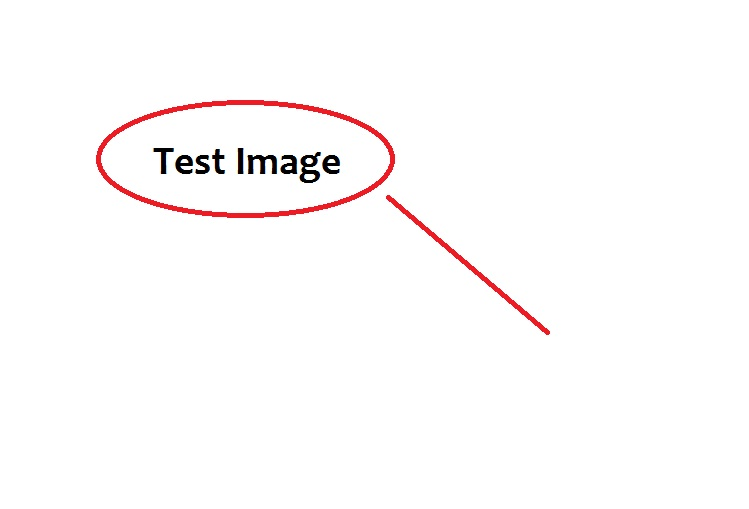
\includegraphics[width=0.8\textwidth]{pic1.jpg}
		\end{center}
		\caption[Caption in List of Figures]{Caption in report}
	\end{figure}


\appendix
	\section{Chase code}
\label{sec:appendix_chase}

	\textbf{TODO: make the long lines short so they fit}
	{\scriptsize
		\lstset{
			language=Haskell,
			numbers=left,
			columns=fixed,
			tabsize=3,
		}
		\lstinputlisting{../chase.hs}
	}



\addcontentsline{toc}{section}{References}
\begin{thebibliography}{9999}

\bibitem{AC}
	A~Cottrell, \textsl{Word Processors: Stupid and Inefficient},\\
	\mbox{} \hfill \url{www.ecn.wfu.edu/\~cottrell/wp.html}

\end{thebibliography}



\end{document}
